\documentclass{beamer}

% Theme choice (you can change to Madrid, CambridgeUS, etc.)
\usetheme{Madrid}

% Optional packages
\usepackage[utf8]{inputenc}
\usepackage{graphicx} % for including images
\usepackage{amsmath, amssymb, mathtools} % for math symbols
\usepackage{hyperref} % for clickable links
\usepackage{tikz}

% Title info
\title[Short Title]{Factor Models of Returns}
\author[Your Name]{Oden Petersen}
\date{\today}

% Section headers
\AtBeginSection[]{
	\begin{frame}
	\vfill
	\centering
	\begin{beamercolorbox}[sep=8pt,center,shadow=True,rounded=True]{title}
		\usebeamerfont{title}\insertsectionhead\par%
	\end{beamercolorbox}
	\vfill
	\end{frame}
}

\begin{document}

% Title page
\begin{frame}
	\titlepage
	\begin{center}
		\textit{``$y=X\beta+\epsilon$, the rest is commentary.''}
	\end{center}
\end{frame}

\begin{frame}{About Me}
\end{frame}

% Table of contents
\begin{frame}{Outline}
	\tableofcontents
	%% Good to include concrete data examples throughout
	%% Make sure := for definitions
\end{frame}

% Section 1
\section{Securities Markets}

\begin{frame}{Spot Transactions}
	The point of trading is to obtain an asset by giving up money, or obtain money by giving up an asset.

	If I give you $q>0$ units of some asset $A$, and you give me $\$p$, then:
	\begin{itemize}
		\item I have \textbf{sold} $q$ units of $A$ to you at $\frac{\$p}{q}$
		\item You have \textbf{bought} $q$ units of $A$ from me for $\frac{\$p}{q}$
	\end{itemize} %"for" and "at" indicate direction

	Buying and selling are collectively called `trading'.

	Suppose I own some amount of $A$ and some amount of money. If we let $s$ be $+1$ for buying and $-1$ for selling, then the result of any trade is to add $qs$ to the amount of $A$ I own, and add $-qps$ to the amount of money I have. %s is called the sign of the trade

	% Stock image of retail store
\end{frame}

\begin{frame}{Securities Markets and Exchanges}
	The \textbf{\textcolor{blue}{market}} is the collective activity of all traders. When we don't care who we trade with, we can just `trade with the market'.

	A \textbf{\textcolor{red}{securities} \textcolor{blue}{market}} for some asset $A$, open at a time $t$, is any \textcolor{red}{standardised} \textcolor{blue}{way for traders to reach agreements to buy or sell} $A$ at a specified \textbf{settlement time} $T\geq t$. %"securities" because of standardisation and regulation. Agreements are often treated as the same as trades, though there are some cases where the distinction matters

	\pause

	For example, $T=\ldots$
	\begin{itemize}
		\item $t$ (`spot', e.g. blockchain) %ASX tried to do blockchain, this was scrapped in 2022 after 7yrs
		\item $t+1, t+2, \ldots$ (`clearing', e.g. equities)
		\item Last Thursday of month (`futures')
	\end{itemize}

	\pause
	If you agree to give something to someone, you have an \textbf{obligation}. If someone agrees to give you something, you have a \textbf{right}.

	\begin{block}{Counterparty Risk}
		If I have an agreement with $P_1$ to buy $10$ units for $\$p_1$ at $T$, and an agreement with $P_2$ to sell $10$ units at $\$p_2$ at $T$, and no further rights/obligations, am I guaranteed to meet my obligations?
	\end{block}%Define counterparty risk
\end{frame}

\begin{frame}{Centralisation}
	A \textbf{securities exchange} is a centralised venue serving a securities market for \textbf{exchange participants} (e.g. ASX, NYSE, TSE, HKEX, LME).

	Agreements not made through an exchange are often called OTC (over-the-counter). %Also called off-exchange. Define search costs.

	\begin{center}
		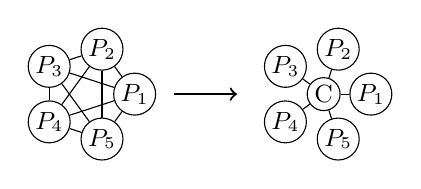
\begin{tikzpicture}[baseline, every node/.style={circle, draw, fill=white, inner sep=1pt, font=\small, minimum size=1mm}]
			\foreach \i in {1,...,5} {
				\node (n\i) at ({72*(\i-1)}:0.6) {$P_{\i}$};
			}
			\foreach \i in {1,...,5} {
				\foreach \j in {1,...,5} {
					\ifnum\i<\j
						\draw (n\i) -- (n\j);
					\fi
				}
			}

			\draw[->, thick] (1.1,0) -- (1.9,0);

			\begin{scope}[xshift=3cm]
				\node (c) at (0,0) {C};
				\foreach \i in {1,...,5} {
					\node (n\i) at ({72*(\i-1)}:0.6) {$P_{\i}$};
					\draw (c) -- (n\i);
				}
			\end{scope}
		\end{tikzpicture}
	\end{center}

	Centralisation generally reduces \textbf{search costs} and \textbf{counterparty risk}. %Mention risk counterexample: FTX vs a DEX
\end{frame}

\begin{frame}{Settlement and Clearing}
	\begin{block}{Netting}
		Centralisation allows for \textbf{netting} of rights and obligations.

		For any settlement time $T$, I only need to keep track of the difference between money owed to and by me, and units owed to and by me.

		The quantity of $A$ owned by me, plus the quantity owed to me, minus the quantity owed by me to others, is known as my \textbf{net position} in $A$. If this is positive, I have a \textbf{long position}. If it is negative, I have a \textbf{short position}. If it is zero, I am \textbf{flat}.
	\end{block}

	\begin{block}{Collateralisation}
		At certain intermediate times $t'$ ($t\leq t'\leq T$), participants may be required to physically give (`post') something to the exchange to \textbf{collateralise} their obligations.
		\begin{itemize}
			\item Money (`margin') %Explain the term "futures type settlement" and "stock type settlement"
			\item Assets (`locate'/`borrow') %"Borrow" is only if you don't own the thing
		\end{itemize}
		If an agreement made on the exchange gives you rights to money or assets, this is typically as good as posting actual money or assets.
	\end{block}
\end{frame}

\begin{frame}{Summary}
	\begin{itemize}
		\item \textbf{Trading} is swapping money and assets
		\item A \textbf{market} is whatever you use to trade
		\item A \textbf{securities market} is a standardised way to agree to trades
		\item Agreements consist of \textbf{rights} and \textbf{obligations}
		\item Finding a \textbf{counterparty} may involve \textbf{search cost}
		\item Agreements between two parties are subject to \textbf{counterparty risk}
		\item A \textbf{securities exchange} is a centralised trading venue %Maybe explain national market system
		\item After trades are agreed to on an exchange, they will be \textbf{settled} in some standardised way
		\item The net quantity of $A$ that I have some claim to can either be positive (\textbf{long position}), negative (\textbf{short position}), or zero (\textbf{flat}).
		\item Traders may be obligated to post assets ('locate') or money ('margin')
	\end{itemize}
\end{frame}

\section{Trading}
\begin{frame}{Setup}
	A sequence of trades that collectively increases the amount of money you have and leaves the amount of each asset you have unchanged is clearly favourable.

	\pause

	Suppose that at each time $t$ we have cash holdings of $\$c_t$ and net holdings of $a_t$ units of some asset $A$.

	Suppose also that trades $(s_t, q_t, \$p_t)$ take place at a finite set of distinct times
	$$\tau = \{t_1,\ldots t_n\}\subset T = [t_-, t_+],$$
	where $t_-<t_1<\ldots<t_n<t_+$.

	\pause

	Suppose further that $p_t$ is a right-continuous function $\mathbb R\to\mathbb R$ with left-limits.

	For instance, we could take $p_t = p_{\max \left(\tau\cap (-\infty,t]\right)}$ for $t\geq \min\tau$ and $p_t=x$ otherwise for some arbitrary $x$. %Last traded price

\end{frame}

\begin{frame}{Accounting}
	Let $c_t^+, a_t^+, p_t^+$ be the right-limits and $c_t^-, a_t^-, p_t^-$ the left-limits of $c_t,a_t, p_t$ respectively.

	\pause

	Define measures $\mathfrak{a}_\omega, \mathfrak{c}_\omega, \mathfrak{p}_\omega$ such that for any interval $T'=[t_-',t_+']$ we have
	$$\mathfrak{a}_{T'} := a_{t_+'}^+-a_{t_-'}^-, \mathfrak{c}_{T'} := c_{t_+'}^+-c_{t_-'}^-, \mathfrak{p}_{T'} := p_{t_+'}^+-p_{t_-'}^-.$$
	Then we have

	\vspace{-0.06\textheight}
	\begin{align*}
		a_{t_+'}^+ - a_{t_-'}^-	&= \sum_{t\in \tau} s_t q_t		&&= \int_{t\in T} d\mathfrak{a},
	\\	c_{t_+'}^+ - c_{t_-'}^-	&= \sum_{t\in \tau} - p_t (s_t q_t)	&&= \int_{t\in T} - p_t d\mathfrak{a},
	\\	p_{t_+'}^+ - p_{t_-'}^- &= p_{t_+'} - p_{t_-'}^-.		&&= \int_{t\in T} d\mathfrak{p}.
	\end{align*}%Special case: t_-'=t_+'
\end{frame}

\begin{frame}{Cash Holdings}
	It can be shown (see appendix) that the cashflow over the entire interval $T=[t_-,t_+]$ is
	$$c_{t_+} - c_{t_-} = \int_{t\in T} - p_t d\mathfrak{a} = p_{t_-}a_{t_-} - p_{t_+}a_{t_+} + \int_{t\in T} a_t^- d\mathfrak{p}.$$
	This is similar in spirit to integration by parts:
	$$\int_a^b f \frac{dg}{dx} dx = f(b)g(b)-f(a)g(a) - \int_a^b g \frac{df}{dx} dx.$$

	Then we have
	$$(c_{t_+} + p_{t_+}a_{t_+}) - (c_{t_-} + p_{t_-}a_{t_-}) = \int_{t\in T} a_t^- dp.$$

	The quantity $\$v_t = \$p_t a_t$ is known as the \textbf{dollar value} of our $A$ holdings \textbf{marked} to the price $\$p_t$.%Marking just means multiplication of units held by a unit price
\end{frame}

\begin{frame}{Portfolio Valuation}
	Suppose now that we trade multiple assets, such that $p_t$, $a_t$ and $v_t$ are vector-valued, with $v_t$ the elementwise product of $p_t$ and $a_t$.

	A collection of assets held in quantities $a_t$ is known as a \textbf{portfolio}.

	\pause

	We can write
	$$(c_{t_+} + p_{t_+} \cdot a_{t_+}) - (c_{t_-} + p_{t_-} \cdot a_{t_-}) = \int_{t\in T} a_t^- \cdot dp,$$
	where $p$ is now a vector-valued measure. \pause Let
	$$\Pi_t	= c_t + p_t\cdot a_t = c_t + \sum v_t.$$

	We call $\$\Pi_t$ the \textbf{value} of our portfolio \textbf{marked} to $p_t$.
\end{frame}

\begin{frame}{Profitability}
	The quantity $\$\Pi_{t_+} - \$\Pi_{t_-}$ is our \textbf{net P\&L} (profit and loss) over the interval $T$, marked to $p_t$.
	Then we have
	$$\Pi_{t_+} - \Pi_{t_-} = \int_{t\in T} a_t^- \cdot dp.$$
	Introducing a measure
	$$\pi_{T'} := \Pi_{t_+'}^+ - \Pi_{t_-'}^-,$$
	we can write
	$$\Pi_{t_{i+1}} - \Pi_{t_i} = \int_{t\in [t_i, t_{i+1}]} d\pi = a_t^- \cdot dp = \int_{t\in [t_i, t_{i+1}]} v_t^- \cdot \frac{dp}{p_t^-},$$
	where $\frac{dp}{p_t^-}$ is the elementwise quotient.
\end{frame}

\begin{frame}{Leverage}
	Suppose we can always make any trade we like at time $t$ with price $\$p_t$. %Not a terrible guess if we did indeed make some trade at $\$p_{t_i}$.

	Then we can freely convert a portfolio with value $\$\Pi_t$ to that much in cash.

	Conversely, we can convert $\$\Pi_t$ worth of cash into any portfolio with that value.

	In practice, there are limits on the trades we can make at a particular price and time.

	\pause

	Typically, $\Pi_t$ can change in two ways: trading assets, or transferring cash into and out of the portfolio. We will generally ignore the possibility of transfers.

	\pause

	If we begin with a portfolio worth $\$\Pi_{t_1}$ and make a sequence of trades of the form $(s_t,q_t,p_t)$ that result in a portfolio worth $\$\Pi_{t_n}$, then we could instead begin with a portfolio worth $L \$\Pi_{t_1}$ and make trades $(s_t, L q_t, p_t)$ to arrive at a portfolio worth $L \$\Pi_{t_n}$. The ratio $L$ is known as the \textbf{leverage ratio}.
\end{frame}

\begin{frame}{Returns}
	Because we typically need money to collateralise some fraction of unsettled trades and short borrow, and hold assets instead of cash, portfolio management requires capital that cannot be used elsewhere.

	In the case of long-only spot-settled trading, if we were to turn our portfolio into cash, or convert cash into an identical portfolio, we would receive/require $\$\Pi_t$.

	\pause

	Consequently, to judge the efficiency of our trading, we might want an estimate for how much extra P\&L over the interval $T$ would result from a marginal dollar added to $\$\Pi_t$.

	\pause

	If our initial portfolio value were $\$\Pi_{t_-}+\$N$ instead of $\Pi_{t_-}$, and we could simply scale up trade sizes at the same prices, then setting
	$$L = \frac{\Pi_{t_-}+N}{\Pi_{t_-}}$$
	means our new P\&L would simply be $L \int_T d\pi$.

	\pause

	The increase in P\&L per dollar added to initial portfolio value is then
	$$R_T = \frac{L \int_T d\pi - \int_T d\pi}{N} = \frac{\int_T d\pi}{\Pi_{t_-}}.$$
	We call $R_T$ the \textbf{return} on the initial portfolio value.
\end{frame}

\begin{frame}{Log Returns}
	If we define
	$$\ell_t = \log \Pi_t$$ %sometimes called log-wealth
	and a measure $\mathfrak{l}_\omega$ satisfying
	$$\mathfrak{l}_{[t_-',t_+']}= \ell_{t_+'}^+ - \ell_{t_-'}^-$$
	for any $t_-',t_+'$, then we have
	$$R_T = \exp(\mathfrak{l}_T) - 1,$$
	and for any measurable set $\omega$ we can define
	$$R_\omega = \exp(\mathfrak{l}_\omega) - 1 \approx \mathfrak{l}_\omega + O(\mathfrak{l}_\omega^2)\textrm{ (for small }\mathfrak{l}_\omega\textrm{)}.$$

	We call $\mathfrak{l}_T$ the \textbf{log-return} over the interval $T$.
\end{frame}

\begin{frame}{Properties of Returns and Log-Returns}
	Let $w_t := \frac{1}{\Pi_t}v_t$ be the \textbf{weight vector}.%Explain interpretation

	For an interval $T' = (t_i,t_{i+1}]$, we have $a_t^-$ equal to a constant over $T'$, and
	$$R_{T'} = w_{t_i}^+ \cdot r_{T'},$$
	where the elementwise quotient
	$$r_{T'} = \frac{p_{t_{i+1}} - p_{t_i}}{p_{t_i}}$$
	is known as the \textbf{asset returns} vector over $T'$. In contrast, $\ell_{T'}$ is not linear in $r_{T'}$. %In fact there's no function of the return that \ell_{T'} is linear in. Benefits and drawbacks, eg expectation/variance

	For a disjoint collection of measurable sets $\omega_1,\ldots\omega_n$ whose union is $\Omega$, we have
	$$\ell_\Omega = \sum_{i=1}^n \ell_{\omega_i},$$
	$$R_\Omega = \left(\prod_{i=1}^n (1+R_{\omega_i})\right) - 1 \approx \sum_{i=1}^n R_{\omega_i} + O\left(\sum_{i=1}^n\sum_{j=1}^n \vert R_{\omega_i} R_{\omega_j} \vert\right).$$
\end{frame}

\begin{frame}{Summary}
	\begin{itemize}
		\item 
	\end{itemize}
\end{frame}

\section{Market Microstructure}
\begin{frame}{Trade Formation}
	In practice, the trades we can make at a time $t$ and a price $p_t$ are limited by our ability to find a willing counterparty.

	\pause
	On an electronic exchange, trades are formed by interacting with the exchange's \textbf{matching engine}.%Matching engine is a computer networked with the computers of exchange participants

	For each trade $(s,q,\$p)$, the exchange will typically charge a fee proportional to the \textbf{dollar volume} $\$pq$ of the trade. Fee rates may vary depending on trade type and between participants in accordance with exchange policy.

	\pause

	The most common type of matching engine design is a \textbf{limit-order book} (sometimes called a double auction), which can operate in either a \textbf{continuous} or \textbf{batched} fashion.
\end{frame}

\begin{frame}{Limit Order Book}%Special kind of data structure
	At any point in time, market participants can create a request (`\textbf{limit order}') of the form $(s,q,\$p)$ to trade up to $q$ units in direction $s=\pm1$ at any price $\$(p-sm), m\geq0$. The value $\$m$ is known as the \textbf{price improvement}. %The request poster prefers large m. $p is sometimes called the reserve price
	
	They are then said to be ``\textbf{bid} for $\$p$'' ($s=+1$) or ``\textbf{ask}ing/\textbf{offer}ing at $\$p$'' ($s=-1$). %Bid and ask are terms referring to limit order directionality. for and at also indicate direction, as mentioned before

	\pause

	All limit orders are collected into a \textbf{limit-order book}.

	Users can add, cancel and modify orders, subject to restrictions.%Limits on modification. Ratelimits, message limits etc. GFD etc - FOK FAK explained later
\end{frame}

\begin{frame}{Order Matching}
	Whenever the book contains orders $(+1,q_1,\$p_1), (-1,q_2,\$p_2)$ with $p_2\leq p_1$, both orders could be at least partly satisfied by trading up to $q_{\max}=\min(q_1,q_2)$ units with one another at a price $\$p\in[\$p_2,\$p_1]$. If such a pair exists the book is said to be \textbf{in cross}.

	\pause

	If an order $(s,q,\$p)$ is in cross with another, it may be \textbf{matched} for $q'$ units. The total matched quantity for all buy orders must equal the total matched quantity for all sell orders.

	\pause

	In this case, $q'$ units will trade, and the order will become $(s,q-q',\$p)$.

	\pause

	If $q=q'$ the order is said to be \textbf{fully filled} and will be removed from the book. Otherwise, it is said to be \textbf{partially filled}.

	\pause
	The ability to quickly find matches for a large number of units at a reasonable price is known as \textbf{liquidity}, and is another major benefit of centralisation.
\end{frame}

\begin{frame}{Supply and Demand Curves}
	Let $\mathcal{L}_t$ be the collection of all limit orders available for trading at time $t$. We can partition this into $\mathcal{L}_t = \mathcal{B}_t\cup\mathcal{A}_t$, with $\mathcal{B}_t$ the bid orders and $\mathcal{A}_t$ the ask orders.

	\pause

	Now define the functions
	\begin{align*}
		Q_t(+1,\$p)	&= \sum_{\substack{(+1,q',\$p') \in \mathcal{B}_t \\ \$p\leq \$p'}} q'
	\\	Q_t(-1,\$p)	&= \sum_{\substack{(-1,q',\$p') \in \mathcal{A}_t \\ \$p\geq \$p'}} q'
	\\	M_t(\$p)	&= \min(Q_t(+1,\$p),Q_t(-1,\$p))
	\end{align*}
	\pause
	The functions $Q_t(-1,\$p)$ and $Q_t(+1,\$p)$ are known as the \textbf{supply curve} and \textbf{demand curve} respectively. The function $M_t(\$p)$ represents the \textbf{matchable quantity} at $\$p$.
	\pause
	The book $\mathcal{L}_t$ is in cross if and only if there exists some $\$p$ with $M_t(\$p)>0$.
	%Diagram. separate slide
\end{frame}

\begin{frame}{Batch Matching}
	In \textbf{batch} or \textbf{auction} style matching, orders are matched with one another only at particular discrete times.

	\pause

	\begin{enumerate}
		\item Prior to the \textbf{match time} $t^*$, users can typically add, modify and cancel limit orders.
		\item At each time $t\leq t^*$, an \textbf{indicative price} $\$p^*_t$ will be selected such that $M_t(\$p^*_t)$ is maximal. Tiebreaking will depend on exchange rules.
		\item Finally, at the match time $t^*$, some subset of the crossed limit orders will be matched at $\$p^*$ for a total quantity $M_{t^*}(\$p^*_{t^*})$. After the match, the book will no longer be crossed.
	\end{enumerate}

	\pause

	Maximising $M_t(\$p^*_t)$ is equivalent to maximising the sum of $qm$ across all orders, where $q$ is the quantity filled and $m$ is the price improvement.%Also maximises fees paid

	It is common to use this matching style at the beginning or end of a trading day or lunch break, or when there is some kind of market instability such as following a large price move or company announcement. Sometimes $t^*$ is referred to as a \textbf{liquidity event} because of the large volume traded, and the relative insensitivity of $\p^*_{t^*}$ to inidividual orders.%Price impact nonnegative because of monotonicity property
\end{frame}

\begin{frame}{Batch Matching Properties}
	The following monotonicity properties typically hold:
	\begin{itemize}
		\item $\$p^*_t$ nondecreasing in $\mathcal{B}_t$ and nonincreasing in $\mathcal{A}_t$
		\item For each $\$p$, $M_t(\$p)$ nondecreasing in $\mathcal{L}_t$
		\item For individual orders $(s,q,\$p)$, we will have $\$p^*_t$ nondecreasing in $\$p$ and $sq$. The sensitivity of $\$p^*_{t^*}$ to $\$p,sq$ is known as \textbf{instantaneous price impact}.
		\item For individual orders $(s,q,\$p)$ and each $\$p'$, we will have $M_t(\$p')$ nondecreasing in $q$ and nondecreasing in $\$sp$.
	\end{itemize}

	\pause

	\begin{block}{Price Priority}
		Because $M_t(\$p')$ is nondecreasing in $sp$, the matching will be designed to obey \textbf{price priority}.
	
		If we have two orders $(s_1,q_1,\$p_1), (s_2,q_2,\$p_2)$ with $\$s_1p_1 > \$s_2p_2$, then the second order cannot be matched unless the first is completely filled.
	\end{block}
\end{frame}

\begin{frame}{Order Timing}
	\begin{block}{Match Time Randomisation}
		Because the order book is often visible to all participants, traders wishing to hide their intentions or make use of all available information may be incentivised to wait until immediately before the match time to post orders.

		To minimise computational throughput requirements for the matching engine, and give more information to all traders, the match time is typically chosen at random in some short interval in order to disincentivise this behaviour.

	\end{block}

	\pause

	\begin{block}{Time Priority}
		To further encourage early submission of orders, many exchanges also implement a time priority rule.%As opposed to pro rata

		If two orders exist at the same price $\$p$, the one that reached the matching engine later cannot be matched unless the earlier order is completely filled.

		This would not have much effect if we could just insert the later order at a price $\$p+s\epsilon$ for some very small $\epsilon>0$.%"Diming"

		To avoid this, prices are only allowed to be integer multiples of some small dollar value $\$\delta$, known as the \textbf{tick size}.%Sub-penny rule reg nms
	\end{block}
\end{frame}

\begin{frame}{Continuous Matching}
	In \textbf{continuous matching}, a match time is triggered every time a new limit order causes the book to become crossed.

	If the matching engine receives an order at $t$, then immediately before and after $t$ the book will be uncrossed, with $M_t(\$p)=0$ at all $\$p$.

	The only orders involved in the match will be the arriving order and some set of orders $\mathcal{M}_t$ in the opposite direction. The arriving order is known as the \textbf{active} or \textbf{aggressive} order, and the pre-existing orders are known as \textbf{passive}. Price priority is still used, and time priority is usually used. %Also known as taker and maker orders. Sometimes have different fees

	% Passive orders provide liquidity to anybody who wants to trade. This liquidity goes away when traded against, so latency matters. Adverse selection comes into play here

	\pause

	Unlike auction-style matching, there may be multiple trade prices according to the prices of the passive orders.

	For each $q'$ matched against a passive order $(s,q,\$p)$, the active order will trade $q'$ units with the passive order at $\$p$. %No price improvement for passive orders

	The per-unit price achieved by the active trader will be
	$$\$p^*_t = \frac{\sum_{(s,q,\$p)\in\mathcal{M}_t} \$pq}{\sum_{(s,q,\$p)\in\mathcal{M}_t} q}.$$ %This may or may not be a multiple of the tick size.

	%Market orders
	%Usually used for intraday trading

	% order priority -> latency -> colocation, fpgas.
	%adverse selection -> order priority. + free messages -> tick size, min size, lot size, ratelimits.
	% "Certainly, the modern compendium of mental illnesses (DSM-5) takes a dim view of people who think everyone is out to get them. Yet financial markets are different: people really are out to get you, after all." - Agustin Lebron, The Laws of Trading

	%FAK,FOK
\end{frame}

\begin{frame}{Price Impact}
	If we aggressively trade a very large quantity, we will exhaust all passive orders we would most prefer to trade with and $\mathcal{M}_t$ will need to include orders at worse price levels. This is sometimes known as \textbf{walking the book}.

	Assume continuous matching, and consider a market order of $q>0$ units in direction $s$. The least favourable price in $\mathcal{M}_t$ will be given by
	$$\$P_t(sq) = s\min_\{(\$p : Q_t(-s,p)\geq q\} \$sp.$$
	The unit price of the match will be given by
	$$\$p^*_t(sq) = \frac{1}{q}\int_0^q \$P_t(sq')dq'.$$

	We call the prices
	\begin{align*}
		\$b_t	&= \lim_{q\to0^+} \$p^*_t(-q)	&&= \max_{(+1,q,\$p)\in\mathcal{B}_t} \$p
	\\	\$a_t	&= \lim_{q\to0^+} \$p^*_t(q)	&&= \min_{(-1,q,\$p)\in\mathcal{A}_t} \$p
	\end{align*}
	the \textbf{bid price} and \textbf{ask price} respectively. All bid orders have price at most $\$b_t$ and all ask orders have price at least $\$a_t$.

	To trade an infinitesimal amount, we would need to sell at $\$b_t$ or buy at $\$a_t$.

	The interval $[\$b_t,\$a_t]$ is known as the \textbf{spread}, and $\$a_t-\$b_t$ is the \textbf{width} of the spread.%Proxy for liquidity

	\pause

	Observe that $\$p^*_t(0)$ is not yet defined. So long as we choose some price $\$m_t$ satisfying $\$m_t\in[\$b_t,\$a_t]$, setting $\$p^*_t(0) := \$m_t$ will make $\$p^*_t(\cdot)$ nondecreasing. This is variously called the \textbf{theo}retical price, \textbf{microprice} or \textbf{price proxy} depending on context.

	Some choices for $m_t$ include:
	\begin{itemize}
		\item $\frac{1}{2}b_t+\$\frac{1}{2}a_t$ (arithmetic \textbf{midprice})
		\item $\$b_t^\frac{1}{2}a_t^\frac{1}{2}$ (\textbf{geometric midprice})
		\item $\$(1-I(\$d))b_t + \$I(\$d)a_t$ (depth-$\$d$ \textbf{weighted midprice}), where $I(\$d)=\frac{Q(+1,\$b_t-\$d)}{Q(+1,\$b_t-\$d)+Q(-1,\$a_t+\$d)}$ is the depth-$\$d$ \textbf{imbalance} (usually $\$d=\$0$)
		\item $\$b_t^{1-I(\$d)}a_t^I(\$d)$ (depth-$\$d$ \textbf{geometrically weighted midprice})
	\end{itemize}

	%bouchaud justification for weighted mid. Most general case is probably: correlated random walks with nonconstant but identical drift,variation

	We call the difference $\lambda_t(sq) = \$p^*_t(sq) - \$m_t$ the \textbf{instantaneous price impact} of trading $q$ units in direction $s$. Buy orders will have nonnegative instantaneous price impact, while sell orders will have nonpositive instantaneous price impact.%Captures everything about liquidity on an immediate timescale

	%Square root law of market impact
	%Gatheral may 19 2016 three models of (persistent) price impact
		%Continuous time propagator: price impact decays according to G()
		%Square root process
		%Alfonso Fruth and Schied: I think the idea is that the shape of the order book above the ask stays the same but the ask changes
		%Locally linear order book
		%Manipulation and transaction-triggered manipulation
		%Optimal liquidation under each model
\end{frame}

\begin{frame}{Market Data \& Market Prices}
	In order to inform trading activity, market participants receive certain data about the orders and trades on the exchange.
	% Theoretical value
		% Efficiency
			%Edge
				%Latency. If you think this is dumb, design a better market that doesnt incentivise it. Hayek quote relevant here
				%PFOF
				%Good pricing
				%Smart order placement (queue rules)
				%Rebates
					%Fee asymmetries
				%Large balance sheet -> higher risk tolerance
				%Funding asymmetry (better funding rates)
				%Alt data
				%Human input -> see things algos dont
				%Better modelling -> see things humans dont
				%Better UI -> algos and humans work together
				%Market access / cross-market synthesis
				%Statistical anomalies/mispricing
		% Liquidity
			% Decomposition of p&l into theo and execution
			% Market maker as liquidity provider
			% Amihud measure? average of |r_day|/daily_volume

	% Price Proxies
		% LTP
			% Price chart. Various position charts.
			% Microstructural noise -> Roll model
		% Midprice, geometric mid
			% Still noisy
		% Weighted mid

	% "lit" exchange just means more market data is made public

	% Order book diagram

\end{frame}

\begin{frame}{Transaction Costs}
	% Fees
	% Spreads
	% Persistent price impact

	% Augmented P&L integral

	% Market impact
		% Adverse selection
		% Trade volumes and liquidity reinforce each other

	%Market making liquidity provision. Avellaneda Stoikov, Crypto AMMs
\end{frame}

\section{Portfolio Management}
\begin{frame}{Uncertainty}
	%Dutch books & FTAP & Q vs P quant. Complete markets, arrow securities. Effects of incompleteness?
		%Dutch books bayes rule?
	%(No-)Arbitrage (buy low sell high. Setup for statarb later)
	%Problems with the notion of probability: 1. estimation (P) 2. market incompleteness (Q) 3. risk premia (Q->P). "All models are wrong" George Box
	%Knightian uncertainty vs quantifiable
	%Estimation problems
		%Empirical risk minimisation
\end{frame}

\begin{frame}{Decision-Making}
	%Systematic, semi-systematic, discretionary
	%High-touch, low-touch
	% What is point of systematic? (consistency, breadth)
		% “We’re mediocre traders, but our system never has rows with its girlfriends — that’s the kind of thing that causes patterns in markets.” Nick Patterson RenTech
\end{frame}

\begin{frame}{Risk}
	% Trading is zero-sum. So why do we do it
	% Risk = variance
		% "Cars have brakes so you can drive faster." Ben Rady
		% Quadratic utility justification. 
	% Portfolio variance and covariance
		%Hedging
\end{frame}

\begin{frame}{Decision Theory}
	%Markowitz frontier
	%Pareto optimality
	%Security market line
	%Markowitz solution
		%Estimation difficulties
	%VNM & kelly theory
\end{frame}

\begin{frame}{Capital Asset Pricing Model}
	% Arbitrage arguments
	% Generalisation to spiked covariance matrix, finite universe. paleologo 7.2.1
	%Efficient Markets
	%Index investing. (Stats?)
		%Why ASX200 and not all ords (microstructure)
		%Grossman-Stiglitz Paradox
\end{frame}

\begin{frame}{Factor Models}
	% Mathematics
		%Cross sectional regression
			%Weighting
		%Factor cov shrinkage (paleologo 6.3.1)
	% Sectors
	% Fama French
	% Factor models approximate cov matrix
		% Why cov matrix approximation is hard to begin with - paleologo 4.5.2 faq 4.5
	% Overrepresentation -> equal weighting (equal weighting index)
	% Factor loadings can't be centred (paleologo 4.4.1) unless an "equal weighting" vector is included
	% Types (paleologo 4.6):
		% characteristic (see paleologo 6.7)
			%Market (1s vector)
			%Countries and industries
			%Momentum
			%Fundamentals
			%Volatility
			%Liquidity
			%Crowding
			%Size
		% statistical
			%Market (beta). Show that this is first principal component
			%Latent factors
				%PPCA = Tipping and Bishop 1998, explicit solution section 3.2. Formulation assumes returns zscored by idio vol, this is not a problem
					%limits to zero paleologo section 7.1.2
		% macroeconomic
			% Fama macbeth
\end{frame}

\begin{frame}{$\alpha$}
	%Spanned vs orthogonal
	%Feature engineering
		%Decays
	%ML
		%Overfitting
			%Regularisation
			%Kitchen sink regression
		%Types
			%Linear
			%Trees
			%Neural nets
			%KNN
			%Genetic algo
			%RL
				%Bellman
		%Hyperparams
			%Gaussian processes
		%Interpretability
			%Peter cotton's point
\end{frame}

\begin{frame}{Statistical Arbitrage}
	% Factor model stat arb (eg pairs trading), kalman filter with factor cov structure
\end{frame}

\section{Options Trading}
	%If black scholes was true options markets wouldnt exist

	%Importance of moneyness as opposed to eg treating options as separate tickers with stationary returns

	% Linear regression mathematics
		% Matrix multiplication
	% Regularisation
	% Factor models in options pricing
		% Diagnosing issues with the model eg because black scholes is wrong ("all models are wrong")

\section{Appendix}
\begin{frame}{Proof Sketch for $\mathfrak{c}_T$ Identity}
	\begin{align*}
			c_{t_+} - c_{t_-}	&= \sum_{t\in\tau} - p_t (s_t q_t)	&&= \sum_{i=1}^n - p_{t_i} (a_{t_i}^+-a_{t_i}^-) = - \sum_{i=1}^n p_{t_i} a_{t_i}^+ + \sum_{i=1}^n p_{t_i} a_{t_i}^-
		\\				&					&&= - \sum_{i=1}^{n-1} p_{t_i} a_{t_{i+1}}^- - p_{t_n} a_{t_n}^+ + \sum_{i=1}^{n-1} p_{t_{i+1}} a_{t_{i+1}}^- + p_{t_1}a_{t_1}^-
		\\				&					&&= p_{t_1}a_{t_1}^- + - p_{t_n} a_{t_n}^+ + \sum_{i=2}^n (p_{t_i}-p_{t_{i-1}}) a_{t_i}^-
		\\				&					&&= p_{t_1}a_{t_1}^- - p_{t_n}a_{t_n}^+ + \int_{t\in[t_1,t_n]} a_t^- d\mathfrak{p}
		\\				&					&&= p_{t_-}a_{t_-} - p_{t_+}a_{t_+} + \int_{t\in T} a_t^- d\mathfrak{p}.
	\end{align*}
\end{frame}

\begin{frame}{Annualised Returns}
	The \textbf{annualised log-return} over $\omega$ is $\ell_\omega \frac{\textrm{1 year}}{\lambda_\omega}$, where $\lambda_\omega$ is the duration (lebesgue measure) of $\omega$ in units of time.%Interpretation. Not defined for instantaneous times

	The \textbf{geometrically annualised return} over $\omega$ is $(1 + R_\omega)^\frac{\textrm{1 year}}{\lambda_\omega} - 1 = \exp\left(\ell_\omega \frac{\textrm{1 year}}{\lambda_\omega}\right) - 1$.

	The \textbf{arithmetically annualised return} over $\omega$ is $R_\omega \frac{\textrm{1 year}}{\lambda_\omega}$. %Approximately same. A bit less meaningful

	%All dimensionless
\end{frame}


\begin{frame}{Stuff I missed}
	% Data cleaning
		%Corporate actions
			% Dividends
			%Stock split, reverse stock split
			%M&A, spinoff
			%Rights issues, tender offer, warrant issue
			%Exchange offer
			%Public offering, share buyback
			%Share buyback
			%Liquidation
			%Delisting
			%Debt to equity conversion
	% How to find alpha
	% How to get a job
	% How to talk to people - traders dont all think so mathematically
	% "People without dirty hands are wrong."
	%Data leakage
		% Survivorship bias / lookahead bias
			%Delisting
		% Corrections added later
		% Redactions or ongoing missingness (the knowledge that it still hasnt been released)
	% Execution algos - TWAP VWAP
	%Backtesting
		%Crossvalidation
		%Walkforward
		%Market impact calibration against live
		%Borrow costs
	%Software design
		%Reproducibility
		%Backtest vs production differences
	%What is a "trading strategy"? What does one "look like"?
		%It's easier to model how markets go right than how they go wrong. All happy families are alike
\end{frame}
\end{document}
